\documentclass[]{article}
\usepackage{lmodern}
\usepackage{amssymb,amsmath}
\usepackage{ifxetex,ifluatex}
\usepackage{fixltx2e} % provides \textsubscript
\ifnum 0\ifxetex 1\fi\ifluatex 1\fi=0 % if pdftex
  \usepackage[T1]{fontenc}
  \usepackage[utf8]{inputenc}
\else % if luatex or xelatex
  \ifxetex
    \usepackage{mathspec}
  \else
    \usepackage{fontspec}
  \fi
  \defaultfontfeatures{Ligatures=TeX,Scale=MatchLowercase}
\fi
% use upquote if available, for straight quotes in verbatim environments
\IfFileExists{upquote.sty}{\usepackage{upquote}}{}
% use microtype if available
\IfFileExists{microtype.sty}{%
\usepackage{microtype}
\UseMicrotypeSet[protrusion]{basicmath} % disable protrusion for tt fonts
}{}
\usepackage[margin=1in]{geometry}
\usepackage{hyperref}
\hypersetup{unicode=true,
            pdftitle={Ancestry estimation based on reference samples of known ethnicities},
            pdfauthor={Hannah Meyer},
            pdfborder={0 0 0},
            breaklinks=true}
\urlstyle{same}  % don't use monospace font for urls
\usepackage{color}
\usepackage{fancyvrb}
\newcommand{\VerbBar}{|}
\newcommand{\VERB}{\Verb[commandchars=\\\{\}]}
\DefineVerbatimEnvironment{Highlighting}{Verbatim}{commandchars=\\\{\}}
% Add ',fontsize=\small' for more characters per line
\newenvironment{Shaded}{}{}
\newcommand{\KeywordTok}[1]{\textcolor[rgb]{0.00,0.44,0.13}{\textbf{#1}}}
\newcommand{\DataTypeTok}[1]{\textcolor[rgb]{0.56,0.13,0.00}{#1}}
\newcommand{\DecValTok}[1]{\textcolor[rgb]{0.25,0.63,0.44}{#1}}
\newcommand{\BaseNTok}[1]{\textcolor[rgb]{0.25,0.63,0.44}{#1}}
\newcommand{\FloatTok}[1]{\textcolor[rgb]{0.25,0.63,0.44}{#1}}
\newcommand{\ConstantTok}[1]{\textcolor[rgb]{0.53,0.00,0.00}{#1}}
\newcommand{\CharTok}[1]{\textcolor[rgb]{0.25,0.44,0.63}{#1}}
\newcommand{\SpecialCharTok}[1]{\textcolor[rgb]{0.25,0.44,0.63}{#1}}
\newcommand{\StringTok}[1]{\textcolor[rgb]{0.25,0.44,0.63}{#1}}
\newcommand{\VerbatimStringTok}[1]{\textcolor[rgb]{0.25,0.44,0.63}{#1}}
\newcommand{\SpecialStringTok}[1]{\textcolor[rgb]{0.73,0.40,0.53}{#1}}
\newcommand{\ImportTok}[1]{#1}
\newcommand{\CommentTok}[1]{\textcolor[rgb]{0.38,0.63,0.69}{\textit{#1}}}
\newcommand{\DocumentationTok}[1]{\textcolor[rgb]{0.73,0.13,0.13}{\textit{#1}}}
\newcommand{\AnnotationTok}[1]{\textcolor[rgb]{0.38,0.63,0.69}{\textbf{\textit{#1}}}}
\newcommand{\CommentVarTok}[1]{\textcolor[rgb]{0.38,0.63,0.69}{\textbf{\textit{#1}}}}
\newcommand{\OtherTok}[1]{\textcolor[rgb]{0.00,0.44,0.13}{#1}}
\newcommand{\FunctionTok}[1]{\textcolor[rgb]{0.02,0.16,0.49}{#1}}
\newcommand{\VariableTok}[1]{\textcolor[rgb]{0.10,0.09,0.49}{#1}}
\newcommand{\ControlFlowTok}[1]{\textcolor[rgb]{0.00,0.44,0.13}{\textbf{#1}}}
\newcommand{\OperatorTok}[1]{\textcolor[rgb]{0.40,0.40,0.40}{#1}}
\newcommand{\BuiltInTok}[1]{#1}
\newcommand{\ExtensionTok}[1]{#1}
\newcommand{\PreprocessorTok}[1]{\textcolor[rgb]{0.74,0.48,0.00}{#1}}
\newcommand{\AttributeTok}[1]{\textcolor[rgb]{0.49,0.56,0.16}{#1}}
\newcommand{\RegionMarkerTok}[1]{#1}
\newcommand{\InformationTok}[1]{\textcolor[rgb]{0.38,0.63,0.69}{\textbf{\textit{#1}}}}
\newcommand{\WarningTok}[1]{\textcolor[rgb]{0.38,0.63,0.69}{\textbf{\textit{#1}}}}
\newcommand{\AlertTok}[1]{\textcolor[rgb]{1.00,0.00,0.00}{\textbf{#1}}}
\newcommand{\ErrorTok}[1]{\textcolor[rgb]{1.00,0.00,0.00}{\textbf{#1}}}
\newcommand{\NormalTok}[1]{#1}
\usepackage{graphicx,grffile}
\makeatletter
\def\maxwidth{\ifdim\Gin@nat@width>\linewidth\linewidth\else\Gin@nat@width\fi}
\def\maxheight{\ifdim\Gin@nat@height>\textheight\textheight\else\Gin@nat@height\fi}
\makeatother
% Scale images if necessary, so that they will not overflow the page
% margins by default, and it is still possible to overwrite the defaults
% using explicit options in \includegraphics[width, height, ...]{}
\setkeys{Gin}{width=\maxwidth,height=\maxheight,keepaspectratio}
\IfFileExists{parskip.sty}{%
\usepackage{parskip}
}{% else
\setlength{\parindent}{0pt}
\setlength{\parskip}{6pt plus 2pt minus 1pt}
}
\setlength{\emergencystretch}{3em}  % prevent overfull lines
\providecommand{\tightlist}{%
  \setlength{\itemsep}{0pt}\setlength{\parskip}{0pt}}
\setcounter{secnumdepth}{0}
% Redefines (sub)paragraphs to behave more like sections
\ifx\paragraph\undefined\else
\let\oldparagraph\paragraph
\renewcommand{\paragraph}[1]{\oldparagraph{#1}\mbox{}}
\fi
\ifx\subparagraph\undefined\else
\let\oldsubparagraph\subparagraph
\renewcommand{\subparagraph}[1]{\oldsubparagraph{#1}\mbox{}}
\fi

%%% Use protect on footnotes to avoid problems with footnotes in titles
\let\rmarkdownfootnote\footnote%
\def\footnote{\protect\rmarkdownfootnote}

%%% Change title format to be more compact
\usepackage{titling}

% Create subtitle command for use in maketitle
\newcommand{\subtitle}[1]{
  \posttitle{
    \begin{center}\large#1\end{center}
    }
}

\setlength{\droptitle}{-2em}

  \title{Ancestry estimation based on reference samples of known ethnicities}
    \pretitle{\vspace{\droptitle}\centering\huge}
  \posttitle{\par}
    \author{Hannah Meyer}
    \preauthor{\centering\large\emph}
  \postauthor{\par}
      \predate{\centering\large\emph}
  \postdate{\par}
    \date{2018-10-24}


\begin{document}
\maketitle

{
\setcounter{tocdepth}{2}
\tableofcontents
}
\section{Ancestry estimation}\label{ancestry-estimation}

The identification of individuals of divergent ancestry can be achieved
by combining the genotypes of the study population with genotypes of a
reference dataset consisting of individuals from known ethnicities (for
instance individuals from the Hapmap or 1000 genomes study {[}1{]}).
Principal component analysis (PCA) on this combined genotype panel can
then be used to detect population structure down to the level of the
reference dataset (for Hapmap and 1000 Genomes, this is down to
large-scale continental ancestry).

In the following, the workflow for combining a study dataset with the
reference samples, conducting PCA and estimating ancestry is
demonstrated. The study dataset consists of 200 individuals and 10,000
genetic markers and is provided with \(plinkQC\) in
\texttt{file.path(find.package(\textquotesingle{}plinkQC\textquotesingle{}),\textquotesingle{}extdata\textquotesingle{})}.

\section{Workflow}\label{workflow}

\subsection{Download reference data}\label{download-reference-data}

A suitable reference dataset should be downloaded and if necessary,
re-formated into PLINK format. Vignettes
\href{https://hannahvmeyer.github.io/plinkQC/articles/HapMap.html}{`Processing
HapMap III reference data for ancestry estimation'} and
\href{}{`Processing 1000Genomes reference data for ancestry
estimation'}, show the download and processing of the HapMap phase III
and 1000Genomes phase III dataset, respectively. In this example, we
will use the HammapIII data as the reference dataset.

\subsection{Set-up}\label{set-up}

We will first set up some bash variables and create directories needed;
storing the names and directories of the reference and study will make
it easy to use updated versions of the reference or new datasets in the
future. Is is also useful to keep the PLINK log-files for future
reference. In order to keep the data directory tidy, we'll create a
directory for the log files and move them to the log directory here
after each analysis step.

\begin{Shaded}
\begin{Highlighting}[]
\VariableTok{qcdir=}\StringTok{'~/qcdir'}
\VariableTok{refdir=}\StringTok{'~/reference'}
\VariableTok{name=}\StringTok{'data'}
\VariableTok{refname=}\StringTok{'HapMapIII'}

\FunctionTok{mkdir}\NormalTok{ -r }\VariableTok{$qcdir}\NormalTok{/plink_log}
\end{Highlighting}
\end{Shaded}

\subsection{Match study genotypes and reference
data}\label{match-study-genotypes-and-reference-data}

In order to compute joint principal components of the reference and
study population, we'll need to combine the two datasets. The plink
--merge function enables this merge, but requires the variants in the
datasets to be matching by chromosome, position and alleles. The
following sections show how to extract the relevant data from the
reference and study dataset and how to filter matching variants.

\subsubsection{Prune study data}\label{prune-study-data}

We will conduct principle component analysis on genetic variants that
are pruned for variants in linkage disequlibrium (LD) with an
\(r^2 >0.2\) in a 50kb window. The LD-pruned dataset is generated below,
using plink --indep-pairwise to compute the LD-variants; additionally
exclude range is used to remove genomic ranges of known high-LD
structure. This file was originally provided by {[}6{]} and is available
in
\texttt{file.path(find.package(\textquotesingle{}plinkQC\textquotesingle{}),\textquotesingle{}extdata\textquotesingle{},\textquotesingle{}high-LD-regions.txt\textquotesingle{})}.

\begin{Shaded}
\begin{Highlighting}[]
\ExtensionTok{plink}\NormalTok{ --bfile  }\VariableTok{$qcdir}\NormalTok{/}\VariableTok{$name}\NormalTok{ \textbackslash{}}
\NormalTok{      --exclude range  }\VariableTok{$refdir}\NormalTok{/}\VariableTok{$highld}\NormalTok{ \textbackslash{}}
\NormalTok{      --indep-pairwise 50 5 0.2 \textbackslash{}}
\NormalTok{      --out }\VariableTok{$qcdir}\NormalTok{/}\VariableTok{$name}
\FunctionTok{mv}  \VariableTok{$qcdir}\NormalTok{/}\VariableTok{$name}\NormalTok{.prune.log }\VariableTok{$qcdir}\NormalTok{/plink_log/}\VariableTok{$name}\NormalTok{.prune}

\ExtensionTok{plink}\NormalTok{ --bfile  }\VariableTok{$qcdir}\NormalTok{/}\VariableTok{$name}\NormalTok{ \textbackslash{}}
\NormalTok{      --extract }\VariableTok{$qcdir}\NormalTok{/}\VariableTok{$name}\NormalTok{.prune.in \textbackslash{}}
\NormalTok{      --make-bed \textbackslash{}}
\NormalTok{      --out }\VariableTok{$qcdir}\NormalTok{/}\VariableTok{$name}\NormalTok{.pruned}
\FunctionTok{mv}  \VariableTok{$qcdir}\NormalTok{/}\VariableTok{$name}\NormalTok{.pruned.log }\VariableTok{$qcdir}\NormalTok{/plink_log/}\VariableTok{$name}\NormalTok{.pruned}
\end{Highlighting}
\end{Shaded}

\subsubsection{Filter reference data for the same SNP set as in
study}\label{filter-reference-data-for-the-same-snp-set-as-in-study}

We will use the list of pruned variants from the study sample to reduce
the reference dataset to the size of the study samples:

\begin{Shaded}
\begin{Highlighting}[]
\ExtensionTok{plink}\NormalTok{ --bfile  }\VariableTok{$refdir}\NormalTok{/}\VariableTok{$refname}\NormalTok{ \textbackslash{}}
\NormalTok{      --extract }\VariableTok{$qcdir}\NormalTok{/}\VariableTok{$name}\NormalTok{.prune.in \textbackslash{}}
\NormalTok{      --make-bed \textbackslash{}}
\NormalTok{      --out }\VariableTok{$qcdir}\NormalTok{/}\VariableTok{$refname}\NormalTok{.pruned}
\FunctionTok{mv}  \VariableTok{$qcdir}\NormalTok{/}\VariableTok{$refname}\NormalTok{.pruned.log }\VariableTok{$qcdir}\NormalTok{/plink_log/}\VariableTok{$refname}\NormalTok{.pruned}
\end{Highlighting}
\end{Shaded}

\subsubsection{Check and correct chromosome
mismatch}\label{check-and-correct-chromosome-mismatch}

The following section uses an awk-script to check that the variant IDs
of the reference data have the same chromosome ID as the study data. For
computing the genetic PC, the annotation is not important, however,
merging the files via PLINK will only work for variants with perfectly
matching attributes. For simplicity, we update the pruned reference
dataset. Note, that sex chromosomes are often encoded differently and
might make the matching more difficult. Again, for simplicty and since
not crucial to the final task, we will ignore XY-encoded sex chromosomes
(via
\texttt{sed\ -n\ \textquotesingle{}/\^{}{[}XY{]}/!p\textquotesingle{}}).

\begin{Shaded}
\begin{Highlighting}[]
\FunctionTok{awk} \StringTok{'BEGIN \{OFS="\textbackslash{}t"\} FNR==NR \{a[$2]=$1; next\} \textbackslash{}}
\StringTok{    ($2 in a && a[$2] != $1)  \{print a[$2],$2\}'}\NormalTok{ \textbackslash{}}
    \VariableTok{$qcdir}\NormalTok{/}\VariableTok{$name}\NormalTok{.pruned.bim }\VariableTok{$qcdir}\NormalTok{/}\VariableTok{$refname}\NormalTok{.pruned.bim }\KeywordTok{|} \KeywordTok{\textbackslash{}}
    \FunctionTok{sed}\NormalTok{ -n }\StringTok{'/^[XY]/!p'} \OperatorTok{>} \VariableTok{$qcdir}\NormalTok{/}\VariableTok{$refname}\NormalTok{.toUpdateChr}

\ExtensionTok{plink}\NormalTok{ --bfile }\VariableTok{$qcdir}\NormalTok{/}\VariableTok{$refname}\NormalTok{.pruned \textbackslash{}}
\NormalTok{      --update-chr }\VariableTok{$qcdir}\NormalTok{/}\VariableTok{$refname}\NormalTok{.toUpdateChr 1 2 \textbackslash{}}
\NormalTok{      --make-bed \textbackslash{}}
\NormalTok{      --out }\VariableTok{$qcdir}\NormalTok{/}\VariableTok{$refname}\NormalTok{.updateChr}
\FunctionTok{mv} \VariableTok{$qcdir}\NormalTok{/}\VariableTok{$refname}\NormalTok{.updateChr.log }\VariableTok{$qcdir}\NormalTok{/plink_log/}\VariableTok{$refname}\NormalTok{.updateChr.log}
\end{Highlighting}
\end{Shaded}

\subsubsection{Position mismatch}\label{position-mismatch}

Similar to the chromosome matching, we use an awk-script to find
variants with mis-matching chromosomal positions.

\begin{Shaded}
\begin{Highlighting}[]
\FunctionTok{awk} \StringTok{'BEGIN \{OFS="\textbackslash{}t"\} FNR==NR \{a[$2]=$4; next\} \textbackslash{}}
\StringTok{    ($2 in a && a[$2] != $4)  \{print a[$2],$2\}'}\NormalTok{ \textbackslash{}}
    \VariableTok{$qcdir}\NormalTok{/}\VariableTok{$name}\NormalTok{.pruned.bim }\VariableTok{$qcdir}\NormalTok{/}\VariableTok{$refname}\NormalTok{.pruned.bim }\OperatorTok{>}\NormalTok{ \textbackslash{}}
    \VariableTok{$qcdir}\NormalTok{/}\VariableTok{$\{refname\}}\NormalTok{.toUpdatePos}
\end{Highlighting}
\end{Shaded}

\subsubsection{Possible allele flips}\label{possible-allele-flips}

Unlike chromosomal and base-pair annotation, mismatching
allele-annotations will not only prevent the plink --merge, but also
mean that it is likely that actually a different genotype was measured.
Initially, we can use the following awk-script to check if non-matching
allele codes are a simple case of allele flips.

\begin{Shaded}
\begin{Highlighting}[]
\FunctionTok{awk} \StringTok{'BEGIN \{OFS="\textbackslash{}t"\} FNR==NR \{a[$1$2$4]=$5$6; next\} \textbackslash{}}
\StringTok{    ($1$2$4 in a && a[$1$2$4] != $5$6 && a[$1$2$4] != $6$5)  \{print $2\}'}\NormalTok{ \textbackslash{}}
    \VariableTok{$qcdir}\NormalTok{/}\VariableTok{$name}\NormalTok{.pruned.bim }\VariableTok{$qcdir}\NormalTok{/}\VariableTok{$refname}\NormalTok{.pruned.bim }\OperatorTok{>}\NormalTok{ \textbackslash{}}
    \VariableTok{$qcdir}\NormalTok{/}\VariableTok{$refname}\NormalTok{.toFlip}
\end{Highlighting}
\end{Shaded}

\subsubsection{Upate positions and flip
alleles}\label{upate-positions-and-flip-alleles}

We use plink to update the mismatching positions and possible
allele-flips identified above.

\begin{Shaded}
\begin{Highlighting}[]
\ExtensionTok{plink}\NormalTok{ --bfile }\VariableTok{$qcdir}\NormalTok{/}\VariableTok{$refname}\NormalTok{.updateChr \textbackslash{}}
\NormalTok{      --update-map }\VariableTok{$qcdir}\NormalTok{/}\VariableTok{$refname}\NormalTok{.toUpdatePos 1 2 \textbackslash{}}
\NormalTok{      --flip }\VariableTok{$qcdir}\NormalTok{/}\VariableTok{$refname}\NormalTok{.toFlip \textbackslash{}}
\NormalTok{      --make-bed \textbackslash{}}
\NormalTok{      --out }\VariableTok{$qcdir}\NormalTok{/}\VariableTok{$refname}\NormalTok{.flipped}
\FunctionTok{mv} \VariableTok{$qcdir}\NormalTok{/}\VariableTok{$refname}\NormalTok{.flipped.log }\VariableTok{$qcdir}\NormalTok{/plink_log/}\VariableTok{$refname}\NormalTok{.flipped.log}
\end{Highlighting}
\end{Shaded}

\subsubsection{Remove mismatches}\label{remove-mismatches}

Any alleles that do not match after allele flipping, are identified and
removed from the reference dataset.

\begin{Shaded}
\begin{Highlighting}[]
\FunctionTok{awk} \StringTok{'BEGIN \{OFS="\textbackslash{}t"\} FNR==NR \{a[$1$2$4]=$5$6; next\} \textbackslash{}}
\StringTok{    ($1$2$4 in a && a[$1$2$4] != $5$6 && a[$1$2$4] != $6$5) \{print $2\}'}\NormalTok{ \textbackslash{}}
    \VariableTok{$qcdir}\NormalTok{/}\VariableTok{$name}\NormalTok{.pruned.bim }\VariableTok{$qcdir}\NormalTok{/}\VariableTok{$refname}\NormalTok{.flipped.bim }\OperatorTok{>}\NormalTok{ \textbackslash{}}
    \VariableTok{$qcdir}\NormalTok{/}\VariableTok{$refname}\NormalTok{.mismatch}

\ExtensionTok{plink}\NormalTok{ --bfile }\VariableTok{$qcdir}\NormalTok{/}\VariableTok{$refname}\NormalTok{.flipped \textbackslash{}}
\NormalTok{      --exclude }\VariableTok{$qcdir}\NormalTok{/}\VariableTok{$refname}\NormalTok{.mismatch \textbackslash{}}
\NormalTok{      --make-bed \textbackslash{}}
\NormalTok{      --out }\VariableTok{$qcdir}\NormalTok{/}\VariableTok{$refname}\NormalTok{.clean}
\FunctionTok{mv} \VariableTok{$qcdir}\NormalTok{/}\VariableTok{$refname}\NormalTok{.clean.log }\VariableTok{$qcdir}\NormalTok{/plink_log/}\VariableTok{$refname}\NormalTok{.clean.log}
\end{Highlighting}
\end{Shaded}

\subsection{Merge study genotypes and reference
data}\label{merge-study-genotypes-and-reference-data}

The matching study and reference dataset can now be merged into a
combined dataset with plink --bmerge. If all steps outlined above were
conducted successfully, no mismatch errors should occur.

\begin{Shaded}
\begin{Highlighting}[]
\ExtensionTok{plink}\NormalTok{ --bfile }\VariableTok{$qcdir}\NormalTok{/}\VariableTok{$name}\NormalTok{.pruned  \textbackslash{}}
\NormalTok{      --bmerge }\VariableTok{$qcdir}\NormalTok{/}\VariableTok{$refname}\NormalTok{.clean.bed }\VariableTok{$qcdir}\NormalTok{/}\VariableTok{$refname}\NormalTok{.clean.bim \textbackslash{}}
         \VariableTok{$qcdir}\NormalTok{/}\VariableTok{$refname}\NormalTok{.clean.fam  \textbackslash{}}
\NormalTok{      --make-bed \textbackslash{}}
\NormalTok{      --out }\VariableTok{$qcdir}\NormalTok{/}\VariableTok{$name}\NormalTok{.merge.}\VariableTok{$refname}
\FunctionTok{mv} \VariableTok{$qcdir}\NormalTok{/}\VariableTok{$name}\NormalTok{.merge.}\VariableTok{$refname}\NormalTok{.log }\VariableTok{$qcdir}\NormalTok{/plink_log}
\end{Highlighting}
\end{Shaded}

\subsection{PCA on the merged data}\label{pca-on-the-merged-data}

We can now run principal component analysis on the combined dataset
using plink --pca which returns a .eigenvec file with the family and
individual ID in columns 1 and 2, followed by the first 20 principal
components.

\begin{Shaded}
\begin{Highlighting}[]
\ExtensionTok{plink}\NormalTok{ --bfile }\VariableTok{$qcdir}\NormalTok{/}\VariableTok{$name}\NormalTok{.merge.}\VariableTok{$refname}\NormalTok{ \textbackslash{}}
\NormalTok{      --pca \textbackslash{}}
\NormalTok{      --out }\VariableTok{$qcdir}\NormalTok{/}\VariableTok{$name}\NormalTok{.}\VariableTok{$reference}
\FunctionTok{mv} \VariableTok{$qcdir}\NormalTok{/}\VariableTok{$name}\NormalTok{.}\VariableTok{$reference}\NormalTok{.log }\VariableTok{$qcdir}\NormalTok{/plink_log}
\end{Highlighting}
\end{Shaded}

\subsection{Check ancestry}\label{check-ancestry}

We can use the .eigenvec file to estimate the ancestry of the study
samples. Identifying individuals of divergent ancestry is implemented in
\texttt{check\_ancestry}. Currently, check ancestry only supports
automatic selection of individuals of European descent. It uses
principal components 1 and 2 to find the center of the known European
reference samples. All study samples whose Euclidean distance from the
centre falls outside the radius specified by the maximum Euclidean
distance of the reference samples multiplied by the chosen
\texttt{europeanTh} are considered non-European.
\texttt{check\_ancestry} shows the result of the ancestry analysis in a
scatter plot of PC1 versus PC2 colour-coded for samples of the reference
populations and the study population. From within R, run the following
command to the ancestry check:

\begin{Shaded}
\begin{Highlighting}[]
\KeywordTok{library}\NormalTok{(plinkQC)}
\NormalTok{package.dir <-}\StringTok{ }\KeywordTok{find.package}\NormalTok{(}\StringTok{'plinkQC'}\NormalTok{)}
\NormalTok{qcdir <-}\StringTok{ }\KeywordTok{file.path}\NormalTok{(package.dir,}\StringTok{'extdata'}\NormalTok{)}
\NormalTok{alg=}\StringTok{'data'}
\NormalTok{refname=}\StringTok{'HapMapIII'}
\NormalTok{refdir=}\StringTok{'~/reference'}


\NormalTok{exclude_ancestry <-}\StringTok{ }\KeywordTok{check_ancestry}\NormalTok{(}\DataTypeTok{qcdir=}\NormalTok{qcdir, }\DataTypeTok{alg=}\NormalTok{alg,}
                            \DataTypeTok{refSamplesFile=}\KeywordTok{paste}\NormalTok{(qcdir, }\StringTok{"/HapMap_ID2Pop.txt"}\NormalTok{,}
                                                 \DataTypeTok{sep=}\StringTok{""}\NormalTok{), }
                            \DataTypeTok{refColorsFile=}\KeywordTok{paste}\NormalTok{(qcdir, }\StringTok{"/HapMap_PopColors.txt"}\NormalTok{,}
                                                 \DataTypeTok{sep=}\StringTok{""}\NormalTok{),}
                            \DataTypeTok{prefixMergedDataset=}\KeywordTok{paste}\NormalTok{(alg, }\StringTok{"."}\NormalTok{, refname,}
                                                      \DataTypeTok{sep=}\StringTok{""}\NormalTok{),}
                            \DataTypeTok{interactive=}\OtherTok{TRUE}\NormalTok{)}
\end{Highlighting}
\end{Shaded}

\begin{center}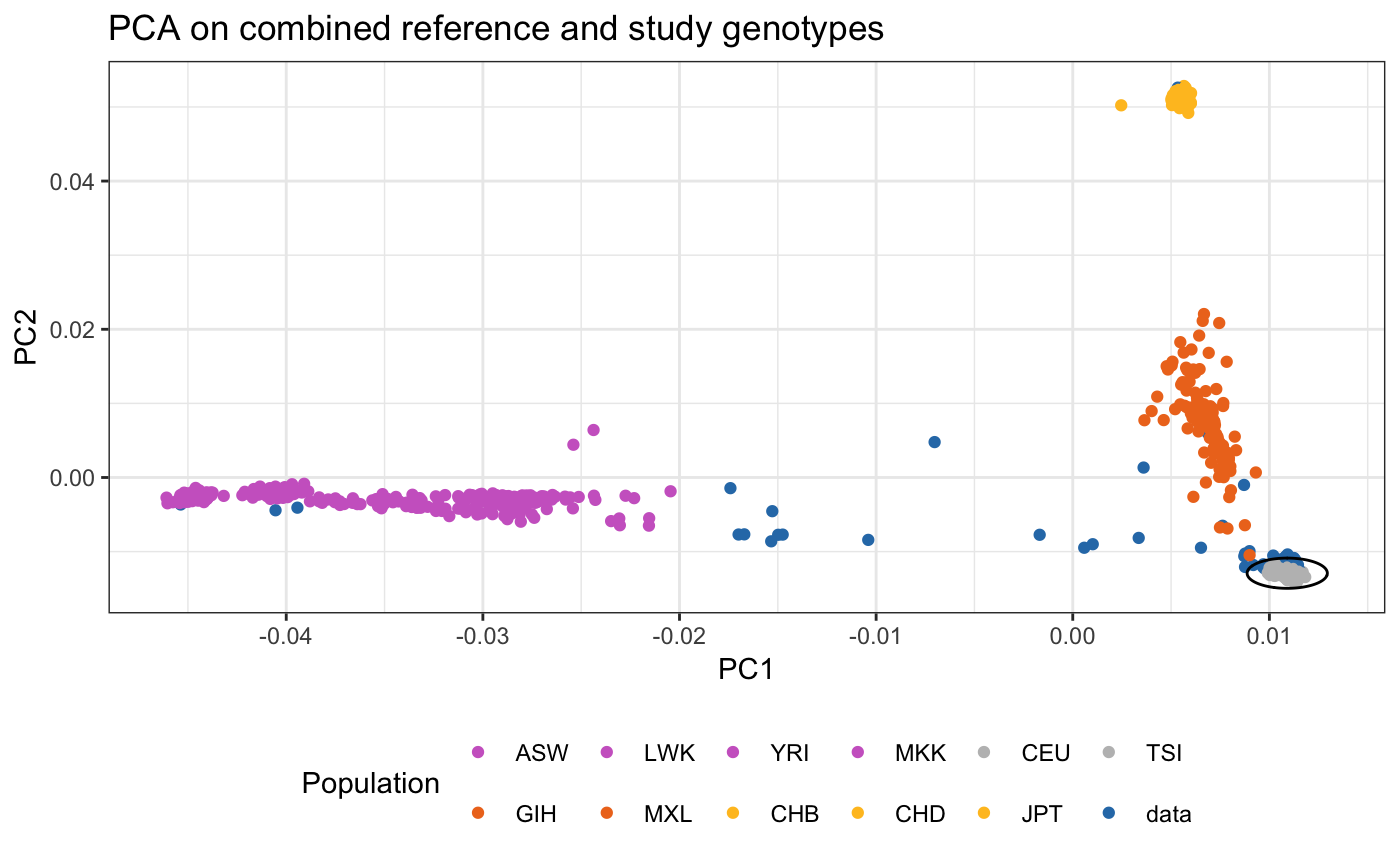
\includegraphics{AncestryCheck_files/figure-latex/check ancestry-1} \end{center}

\section*{References}\label{references}
\addcontentsline{toc}{section}{References}

\hypertarget{refs}{}
\hypertarget{ref-HapMap2005}{}
1. The International HapMap Consortium. A haplotype map of the human
genome. Nature. 2005;437: 1299--320.
doi:\href{https://doi.org/10.1038/nature04226}{10.1038/nature04226}

\hypertarget{ref-HapMap2007}{}
2. The International HapMap Consortium. A second generation human
haplotype map of over 3.1 million SNPs. Nature. 2007;449: 851.
doi:\href{https://doi.org/10.1038/nature06258}{10.1038/nature06258}

\hypertarget{ref-HapMap2010}{}
3. The International HapMap Consortium. Integrating common and rare
genetic variation in diverse human populations. Nature. 2010;467.
doi:\href{https://doi.org/10.1038/nature09298}{10.1038/nature09298}

\hypertarget{ref-a1000Genomes2015}{}
4. 1000 Genomes Project Consortium. An integrated map of structural
variation in 2,504 human genomes. Nature. 2015;526: 75--81.
doi:\href{https://doi.org/10.1038/nature15394}{10.1038/nature15394}

\hypertarget{ref-b1000Genomes2015}{}
5. 1000 Genomes Project Consortium. A global reference for human genetic
variation. Nature. 2015;526: 75--81.
doi:\href{https://doi.org/10.1038/nature15393}{10.1038/nature15393}

\hypertarget{ref-Anderson2010}{}
6. Anderson CA, Pettersson FH, Clarke GM, Cardon LR, Morris AP,
Zondervan KT. Data quality control in genetic case-control association
studies. Nature Protocols. 2010;5: 1564--73.
doi:\href{https://doi.org/10.1038/nprot.2010.116}{10.1038/nprot.2010.116}


\end{document}
